\documentclass[10pt,a4paper]{article}
\usepackage[a4paper,margin=22mm,top=32mm,bottom=26mm,headheight=16mm]{geometry}
\usepackage{fontspec}
\setmainfont{Helvetica Neue}
\usepackage{graphicx,xcolor,booktabs,tabularx,array,fancyhdr,lastpage,titlesec,enumitem,float,microtype,hyperref}
\definecolor{ink}{HTML}{111827}\definecolor{muted}{HTML}{6B7280}\definecolor{cb}{HTML}{2D6BFF}\definecolor{rule}{HTML}{D1D5DB}\definecolor{panel}{HTML}{F3F6FF}
\hypersetup{colorlinks=true,urlcolor=cb,linkcolor=ink}
\color{ink}
\setlength{\parindent}{0pt}\setlength{\parskip}{6pt}
\titleformat{\section}{\Large\bfseries}{}{0pt}{}[{\color{rule}\titlerule}]
\titleformat{\subsection}{\large\bfseries}{}{0pt}{}
\titlespacing*{\section}{0pt}{16pt}{8pt}
\renewcommand{\arraystretch}{1.25}
\newcolumntype{R}{>{\raggedleft\arraybackslash}X}

\pagestyle{fancy}\fancyhf{}
\renewcommand{\headrulewidth}{0.4pt}\renewcommand{\footrulewidth}{0.4pt}
\renewcommand{\headrule}{\hbox to\headwidth{\color{rule}\leaders\hrule height \headrulewidth\hfill}}
\renewcommand{\footrule}{\hbox to\headwidth{\color{rule}\leaders\hrule height \footrulewidth\hfill}}
\fancyhead[L]{\raisebox{-3pt}{
\includegraphics[height=9mm]{figures/emblem.pdf}}\hspace{2mm}{\bfseries\large Cognoscenti}}
\fancyhead[R]{\color{muted}\small Memory Trustworthiness Benchmark Report\\ Run of 24 November 2026}
\fancyfoot[L]{\color{muted}\small Cognoscenti benchmark report}
\fancyfoot[C]{\color{muted}\small\thepage\ of \pageref{LastPage}}
\fancyfoot[R]{\color{muted}\small\href{https://achiral.ai/cognoscenti}{achiral.ai/cognoscenti}}

\newcommand{\fig}[2]{\begin{figure}[H]\centering\includegraphics[width=\linewidth]{figures/#1.pdf}\par\vspace{2pt}{\color{muted}\small #2}\end{figure}}

\begin{document}
\thispagestyle{empty}
\begin{center}
\vspace*{18mm}

\includegraphics[height=34mm]{figures/emblem.pdf}\\[6mm]
{\fontsize{34}{38}\selectfont\bfseries Cognoscenti}\\[3mm]
{\Large\color{muted} An open benchmark for trustworthy AI memory}\\[16mm]
{\fontsize{24}{28}\selectfont\bfseries Memory Trustworthiness\\Benchmark Report}\\[6mm]
{\large Achiral Memory API against retrieval baselines}\\[3mm]
{\color{muted} Run of 24 November 2026\quad·\quad 544 questions\quad·\quad 5 replicates}\\[18mm]
\colorbox{panel}{\parbox{0.82\linewidth}{\centering\vspace{6mm}
{\fontsize{54}{58}\selectfont\bfseries\color{cb}0.88}\\[1mm]
{\large Memory Trustworthiness, 95\% interval 0.85 to 0.90}\\[3mm]
{\small No private note leaked in 141 trials\ \ ·\ \ best baseline (bm25) scores 0.63\vspace{6mm}}}}
\end{center}
\vfill
{\color{muted}\small Provenance: Achiral serving commit \texttt{5a11cad}; Cognoscenti binary \texttt{3a76bf1};\\ stream \texttt{trust-seed-0}, sha256 \texttt{2fc8d6c2…93e2}.}
\newpage

\section{Summary}
Cognoscenti scores whether an AI memory system can be trusted with a team's information. This report gives the first Memory Trustworthiness score for the Achiral Memory API and sets it beside five baselines scored the same way on the same stream.

\begin{itemize}[leftmargin=1.2em,itemsep=2pt]
\item \textbf{Memory Trustworthiness is 0.88} (95\% interval 0.85 to 0.90) for Achiral. The best baseline, bm25 keyword search, scores 0.63.
\item \textbf{Access is 1.00.} Achiral returned no private note to the wrong actor in 141 trials. With zero leaks the leak rate is below 2.1\% (the 3/n bound). bm25 leaked in 88\% of the same trials.
\item \textbf{Currency is 1.00.} In all 70 supersede trials the current fact beat the one it replaced.
\item \textbf{Recall is 0.90} (0.86 to 0.93), level with the best baseline on this component (verbatim 0.90, bm25 0.87).
\item \textbf{Private memory is 0.61} (0.52 to 0.69). It is the weakest of the four. bm25 scores 0.95 there only because it returns everything it holds, including what it should not.
\item \textbf{Cost:} Achiral injects 27.3 words of memory per question, against 9,447.8 for full context (about 350 times fewer) and 31.8 for bm25.
\end{itemize}

\textbf{Read this first.} The retrieval setting in this result (keyword candidates added to the rerank) was chosen after a first run on the same stream scored 0.80. Both runs are reported in Section 6 and should be read as one tuned system, not two independent tests. The 316 trials that need per-member accounts were not run. Calibration is derived from each system's ranking, not stated by the system.

\section{1\quad What Memory Trustworthiness measures}
Memory Trustworthiness is the unweighted mean of four component scores, each between 0 and 1.

\begin{tabularx}{\linewidth}{@{}lXr@{}}
\toprule
Component & What it asks & Trials\\\midrule
Access & Does a private note stay private? One minus the leak rate over scope and agent trials. & 141\\
Currency & When a fact is replaced, does the current one win? & 70\\
Recall & Is the right note in the top three, for plain, paraphrased, reworded and stable questions? & 280\\
Private memory & Does the system still find a user's own agent, owner and individual notes? & 123\\\bottomrule
\end{tabularx}

\textbf{Method.} The stream \texttt{trust-seed-0} was generated with seed 0 and lints clean. Achiral was replayed through its public API five times, each in a fresh organization, at top-3. Baselines (\texttt{verbatim}, \texttt{bm25}, \texttt{recency}, \texttt{full-context}, \texttt{bounded-window}) ran through the same harness and the same formula, also at five replicates. Every interval is a 95\% percentile bootstrap (10,000 draws) over questions. Where a component has no events, the 3/n rule-of-three bound is used instead.

\textbf{Display rule.} A Memory Trustworthiness number is shown only with its four components, trial counts, intervals, the baselines, the run date, the serving commit and the stream hash.

\clearpage
\section{2\quad Results}
\fig{fig1_score}{Figure 1. Memory Trustworthiness by system. Full-context and bounded-window score 0.00 because they cannot find a specific note.}

\begingroup\small\setlength{\tabcolsep}{4pt}\begin{tabular}{@{}lrrrrr@{}}
\toprule
System & Trust & Access & Currency & Recall & Private\\\midrule
\textbf{Achiral} & \textbf{0.88} (0.85--0.90) & \textbf{1.00} & \textbf{1.00} & 0.90 (0.86--0.93) & 0.61 (0.52--0.69)\\
bm25 & 0.63 (0.60--0.67) & 0.12 & 0.60 & 0.87 & 0.95\\
recency & 0.50 & 0.00 & 1.00 & 0.00 & 1.00\\
verbatim & 0.47 (0.44--0.50) & 0.60 & 0.00 & 0.90 & 0.41\\
bounded-window & 0.00 & 0.00 & 0.00 & 0.01 & 0.00\\
full-context & 0.00 & 0.00 & 0.00 & 0.01 & 0.00\\\bottomrule
\end{tabular}\endgroup
{\color{muted}\small n: Access 141, Currency 70, Recall 280, Private memory 123, questions 544. Intervals shown for Achiral and where they are not degenerate.}

\fig{fig2_components}{Figure 2. The four components by system. Whiskers are 95\% intervals. A baseline that returns everything scores high on Private memory only because it leaks; read it beside Access.}

\section{3\quad The axes of trust}
Cognoscenti tests trust along three axes: scope, stability and calibration. A fourth axis, cost, is in Section 4.

\subsection*{Scope: does it respect the boundaries it is told?}
\fig{fig3_scope}{Figure 3. Private-note leak rate over 141 scope and agent trials. The baselines ignore actor scope, so their rows are controls, not secure systems.}
Achiral leaked in 0 of 71 scope trials and 0 of 70 agent trials, in every one of five replicates. The bound is below 2.1\% for the 141 trials together.

\subsection*{Stability: does it agree with itself when repeated?}
\fig{fig4_stability}{Figure 4. Questions fully recalled in each of five fresh replicates, both arms.}
Arm 2 recalled 466 or 467 of 544 questions in every replicate. Four questions changed their outcome across replicates (a flip rate of 0.7\%). The deterministic baselines never flip.

\subsection*{Calibration: does its confidence mean anything?}
\begin{minipage}[t]{0.46\linewidth}\vspace{0pt}
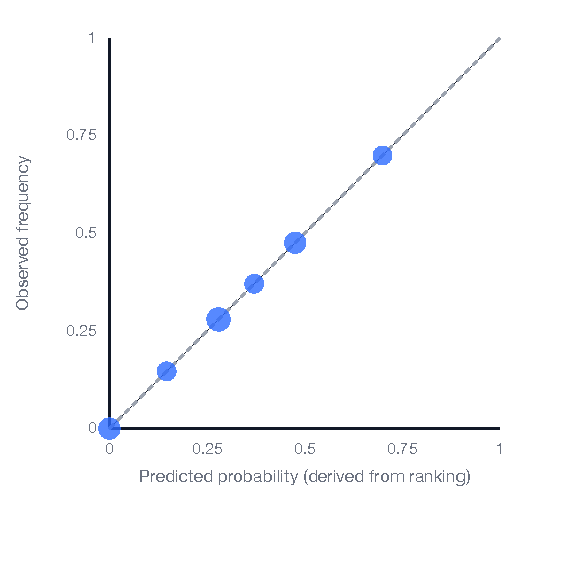
\includegraphics[width=\linewidth]{figures/fig5_calibration.pdf}
\end{minipage}\hfill
\begin{minipage}[t]{0.50\linewidth}\vspace{0pt}
{\color{muted}\small Figure 5. Reliability diagram, arm 2.}

\medskip
Achiral's expected calibration error is near zero (Brier 0.168). \textbf{This is weak evidence.} Cognoscenti derives the predicted probability from each system's ranking, so the points sit on the diagonal by construction. A system that states its own confidence is the stronger test, and Achiral is not yet scored that way.
\end{minipage}

\section{4\quad Cost: tokens injected per question}
\fig{fig6_tokens}{Figure 6. Tokens injected into the model per question (left, log scale) and Memory Trustworthiness against tokens (right).}
\begin{tabularx}{\linewidth}{@{}lRR@{}}
\toprule
System & Tokens per question (95\% interval) & Compared with Achiral\\\midrule
\textbf{Achiral} & \textbf{27.3} (26.6--27.9) & ---\\
verbatim & 29.9 (29.1--30.7) & 1.1 times\\
recency & 30.0 (29.5--30.5) & 1.1 times\\
bm25 & 31.8 (31.1--32.5) & 1.2 times\\
bounded-window & 160.5 (159.2--161.8) & 5.9 times\\
full-context & 9,447.8 (8,989.6--9,914.9) & 347 times\\\bottomrule
\end{tabularx}

Against full context, Achiral injects about 99.7\% fewer tokens and scores 0.88 where full context scores 0.00. Against the other top-k retrievers the saving is small (9 to 14\%), and those systems score lower on trust. Tokens here are whitespace-separated words on the read path only. Ingestion cost is not measured. \textbf{Not measured:} how tokens change over repeated cycles of use (the ``durable horizon'' axis). The runner exists and no Achiral run has been done.

\section{5\quad Where Achiral loses points}
Recall by question category, arm 2 (mean recall at three over five replicates):
paraphrase 1.00, scope 1.00, supersede 1.00, owner 1.00 (n=18), retrieve 0.89, stable 0.89, rephrase 0.81, agent 0.57 (n=70), individual 0.49 (n=35).

The two weakest categories are both private memory: notes an agent or an individual wrote for themselves. Achiral's agent-scope route was found to ignore note timing and replacement, so a replaced agent note could still rank. A fix is built and tested (event time and supersession on agent notes), \textbf{but it is not part of this run} and is not yet measured.

\section{6\quad Two arms, and what changed between them}
\fig{fig7_arms}{Figure 7. Arm 1 (0.80) and arm 2 (0.88), same stream and serving commit.}
Arm 2 sends \texttt{keywordCandidates}, which adds keyword-matched notes to the candidates the reranker sees. Nothing else differs. Currency rose from 0.86 to 1.00, Recall from 0.88 to 0.90 and Private memory from 0.46 to 0.61. Access stayed at 1.00.

\textbf{The setting was chosen after seeing arm 1 on this same stream.} The two arms are one tuned system, and the 0.88 is not a clean held-out test. A fair test needs a stream that did not shape the settings.

\fig{fig8_categories}{Figure 8. Recall by category, arm 1 and arm 2.}

\section{7\quad Limits}
\begin{itemize}[leftmargin=1.2em,itemsep=2pt]
\item \textbf{Per-member accounts are not run.} 316 trials that need user-scope routes (scope 229, individual 35, owner 52) are excluded, because a refused write must not count as ``nothing leaked''. The figures cover agent and organization scope.
\item \textbf{One synthetic stream.} Questions come from one generator and one seed. Results on real team data are not shown.
\item \textbf{Tuned on this stream.} See Section 6.
\item \textbf{Baselines are controls.} \texttt{bm25} and \texttt{verbatim} ignore actor scope; they show what retrieval does without access control, not a competing secure product.
\item \textbf{Tokens} count words on the read path, not model tokens, and ignore ingestion.
\item \textbf{Calibration} is derived from ranking.
\item \textbf{Hardware.} The host slept for part of the run (about 6 h 41 min of a 14 h 31 min wall time for arm 2, from the power log). The server and harness did not restart and no score depends on wall-clock time.
\end{itemize}

\section{8\quad Provenance and reproduction}
\begin{tabularx}{\linewidth}{@{}lX@{}}
\toprule
Item & Value\\\midrule
Run (arm 2) & 2026-11-24, 03:46 to 18:17 UTC; exit 0\\
Achiral serving commit & \texttt{5a11cad76aecc4badcb8a7de5bff86c24fec6da4}; container restarted 0 times, same start time at the end\\
Cognoscenti binary & \texttt{cognoscenti-3a76bf1}\\
Stream & \texttt{trust-seed-0}, sha256 \texttt{2fc8d6c2…f5693e2}\\
Settings & 5 replicates, seed 0, top-3, \texttt{-{}-skip-user-scope}, 15 s settle, 10 min confirm budget, fresh organization per replicate\\
Baselines & Same binary and stream, 5 replicates, run 2026-11-24 (earlier 3-replicate figures were identical)\\
Scoring & Unweighted mean of four components; 95\% percentile bootstrap, 10,000 draws\\\bottomrule
\end{tabularx}

\textbf{Source and record.} Code and results: \href{https://github.com/Achiral-AI/cognoscenti}{github.com/Achiral-AI/cognoscenti}. Preregistration with dated result notes for both arms: \texttt{docs/preregistration-memory-trustworthiness-2026-11.md}. Page: \href{https://achiral.ai/cognoscenti}{achiral.ai/cognoscenti}.
\end{document}
